\section{REPRESENTAÇÃO DOS INDIVÍDUOS}
\label{sec:2representacao}

Os \acp{AG} diferem da \ac{PG} essencialmente pela forma como os indivíduos são 
representados e codificados. Nos \acp{AG}, os indivíduos são representados por uma cadeia fixa de caracteres 
(geralmente binários), tal como ilustrado na \figref{Figura221}.

%\begin{figure}[H]
%	\centering
%	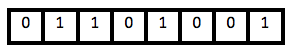
\includegraphics[width=0.5\textwidth]{figures/2}
%	\caption{Representação de um indivíduo em cadeia de caracteres binários}
%	\label{Figura221}
%\end{figure}
\vspace*{1mm}
\begin{figure}[H]
	\centering
	\makebox[\textwidth]{} \par
	\fbox{$0$}\fbox{$1$}\fbox{$1$}\fbox{$0$}\fbox{$1$}\fbox{$0$}\fbox{$0$}\fbox{$1$}
	\caption{Representação de um indivíduo em cadeia de caracteres binários}
	\label{Figura221}
\end{figure}
\vspace*{1mm}

A representação em cadeia fixa de caracteres carece de uma propriedade importante e usualmente encontrada nas soluções de 
problemas complexos: a organização hierárquica das soluções em tarefas e subtarefas \citep{Koza1992}. Para além desta deficiência, 
outras foram levantadas em \citep{DeJong1985} e \citep{Koza1992}.

Na \ac{PG} os indivíduos são programas de computador. Estes indivíduos são geralmente representados em árvores de 
sintaxe, mas existem outras formas de representação como por exemplo: linear \citep{Banzhaf1993,Kinnear:Nordin}, 
em grafo \citep{Poli:1996:nnPDGP,Teller:1996:aigp2} e cartesiana \citep{MS:IEEETEC:06,miller:1999:ACGP}. 
Neste trabalho adoptou-se a representação mais comum: árvores de sintaxe \citep{Koza1992}.

As árvores de sintaxe são construídas a partir de um conjunto de funções \\
$F=\{f_1,\ldots,f_n\}$ que representam os nós da árvore
e um conjunto de símbolos terminais $T=\{t_1,\ldots,t_n\}$ que representam as folhas da árvore. 
Assim, o espaço de procura de soluções é constituído por todas as expressões que podem ser construídas recursivamente com as 
funções em $F$ e os símbolos terminais em $T$. 

Cada função do conjunto $F$ pode ser uma função aritmética, matemática, lógica ou outra, que aceite um determinado número de 
argumentos (aridade) \citep{Koza1992}. Um elemento do conjunto $T$ pode ser uma variável ou uma constante definida sobre o 
domínio do problema. A \figref{Figura222}, apresenta uma árvore válida construída “aleatoriamente” a partir dos conjuntos $F=\{{+,-,*,/}\}$ 
e $T=\{{x_1,x_2}\}$.

\begin{figure}[H]
	\centering
	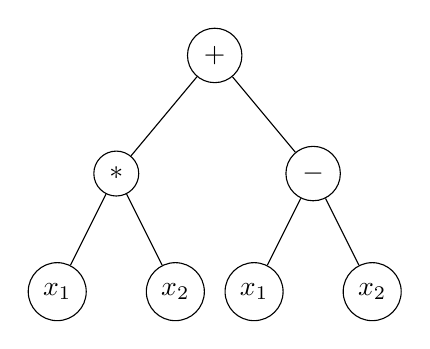
\begin{tikzpicture}[every node/.style={circle,draw}] 
    	\tikzstyle{level 1}=[sibling distance=2.5cm] 
    	\tikzstyle{level 2}=[sibling distance=1.5cm] 
    	\node {$+$}
	    child{node {$*$} child{node {$x_1$}} child{node {$x_2$}}}
	    child{node {$-$} child{node {$x_1$}} child{node {$x_2$}}};
	\end{tikzpicture}%
	\caption{Exemplo de um indivíduo em \ac{PG}}
	\label{Figura222}
\end{figure}

Esta árvore corresponde a expressão matemática,

\begin{equation}
f(x_1,x_2) = (x_1*x_2) + (x_1-x_2)
\label{Equacao221}
\end{equation}

As funções em $F$ devem obedecer a propriedade do fechamento para garantir consistência nos tipos de dados e segurança na avaliação 
das expressões por elas criadas \citep{Poli2008}. Considerando a expressão da \equationref{Equacao221} que representa o 
indivíduo da \figref{Figura222}, a consistência 
nos tipos de dados consiste em garantir que os valores para as variáveis $x_1$ e $x_2$ estejam definidos para os operadores de 
adição ($+$) e subtração ($-$). Mesmo respeitando esta propriedade algumas funções podem falhar ao serem executadas. 
Um caso comum, é a divisão por $0$. Koza introduziu uma nova operação, a divisão protegida (${\%}$), que retorna o valor $1$ sempre que 
o denominador for igual a $0$ \citep{Koza1992}.

Os elementos dos conjuntos $F$ e $T$ devem ser suficientes para representar as soluções do problema dado. Esta propriedade de 
suficiência, nem sempre é satisfeita porque antes da execução do algoritmo a estrutura da solução não é conhecida, e logo, não há 
garantia que os elementos em $F$ e $T$ sejam suficientes para representar a solução do problema. Um exemplo de um conjunto suficiente é o conjunto $F =\{{AND,OR,NOT}\}$ que só 
por si é adequado para representar qualquer função \emph{booleana} \citep{Koza1992}.